To visualize the relationships within the model, we harnessed the power of
Graphviz, an open source graph visualization software. Graphviz uses a simple
text file format that indicates relationships between nodes, and outputs a
variety of image formats.\par
Once the initial hurdles of communication were overcome, we were able to agree
on how we wanted the graph to look, and the resulting graphs accurately portray
the relationships of the memory model used in our analysis.\par
When an analysis has been completed, a call is made to dump the current contents
of the memory. We the pointers to location objects as node keys in the graph and
label the contents of each node accordingly.\par
Having already built the location relationships, we simply traverse the
relationships, outputting as we go. As previously discussed, each location has a
clearly defined child-parent relationship, so we only need to call the graph
function on the root \texttt{Proc\_Loc}.\par
When the graph function is called on the root \texttt{Proc\_Loc} (typically, this
is the \texttt{main} function), each child of that \texttt{Proc\_Loc} is a
\texttt{BB\_Loc}, so it's matter of stepping through each child and outputting
the relationship accordingly. Since the nodes are indexed by pointers, it's a
reasonably straight-forward task. Following the display of all the
\texttt{Proc\_Loc} to \texttt{BB\_Loc} relationships, a graph function is called
on each \texttt{BB\_Loc}.\par
At each \texttt{BB\_Loc}, the statements within are assigned to the
\texttt{BB\_Loc} in a tabular format, as well as added to a queue. Following the
processing of all the statements within a \texttt{BB\_Loc}, the queue is
processed. Each element in the queue is a \texttt{Stmt\_Loc}, and a graph
function is called in it.\par
The graph function for a \texttt{Stmt\_Loc} is very simple. If the statement is a
call-site, the child will point to a \texttt{Proc\_Loc}. In this case, the graph
function is called on the child \texttt{Proc\_Loc}. Otherwise, the graphing
processes stops there.\par
Although the original intent of the graph was to incorporate definitions and
usages, time constraints limited the success of incorporating the information
obtained from the \texttt{Mem\_Table} into the graph. The chain of graphing
functions exist, but we not completed by the deadline.\par
To illustrate what the current visualization looks like, we'll take the
following code block:
\lstset{%
  basicstyle=\small,
  language=C,
  stringstyle=\ttfamily,
  showstringspaces=false,
  linewidth=\textwidth,
  tabsize=2,
  captionpos=b
}
\begin{lstlisting}
int* identity (int* in) {
  int *out = in;
  *out = 222;
  return out;
}

int main () {
  int data = 111;
  int data2= 333;
  int *ptr = data == 2 ? &data : &data2;

  *ptr = 222;

  int copy_of_data = *ptr;

  int *clone_ptr;
  clone_ptr = identity(ptr);

  *clone_ptr = 333;
}
\end{lstlisting}

Here, running the visualization gives us Figure \ref{fig:passes4-vis}.

\begin{figure}
\begin{center}
\leavevmode
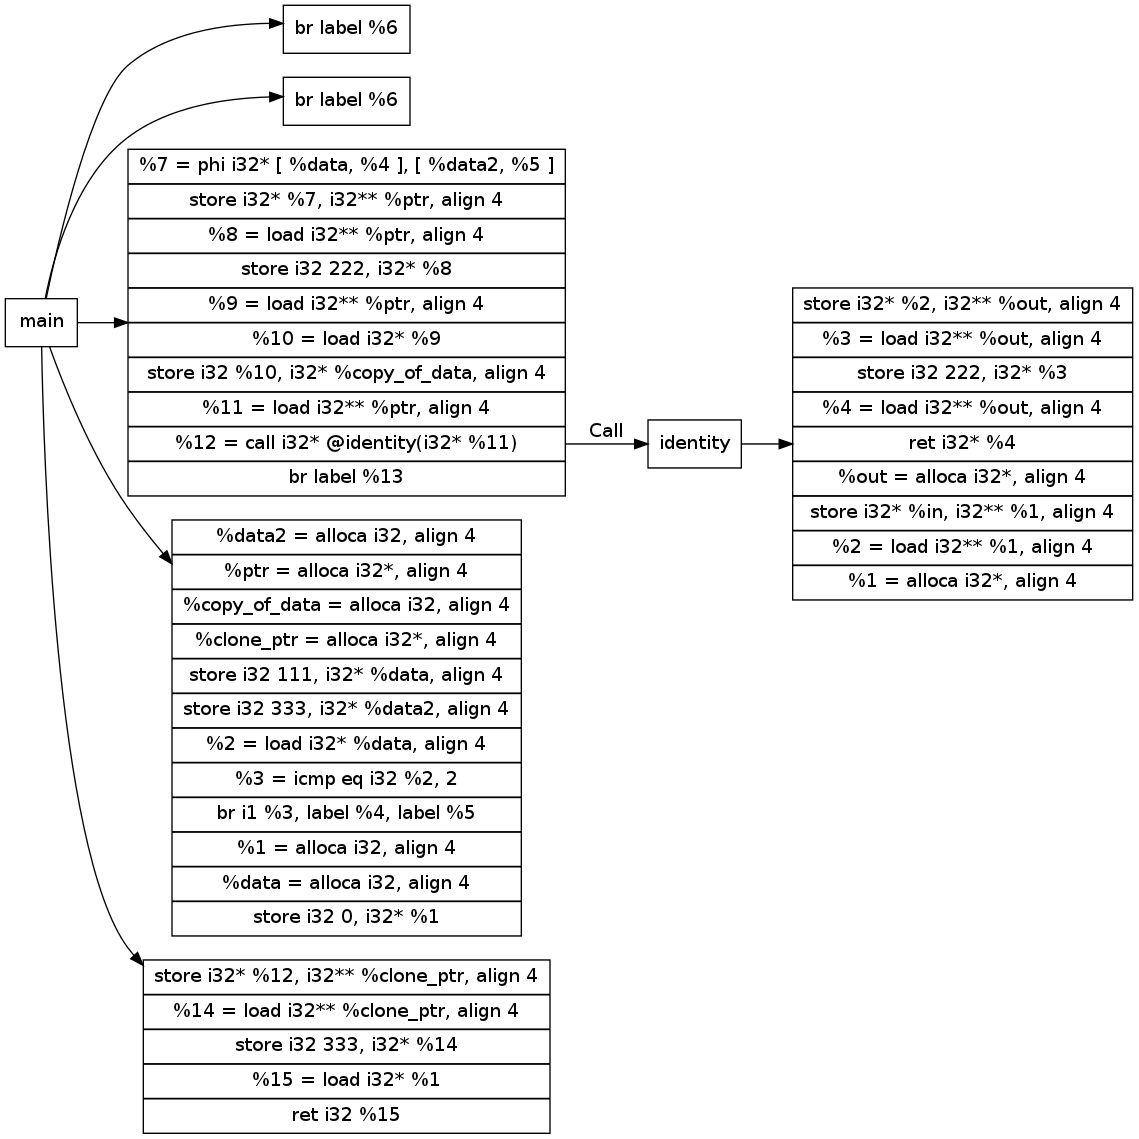
\includegraphics[scale=0.4]{images/passes4.png}
\end{center}
\caption{Example Visualization of a Code Block}
\label{fig:passes4-vis}
\end{figure}
